\documentclass[11pt]{article}

\usepackage{graphicx}
\usepackage{framed}

% Use wide margins, but not quite so wide as fullpage.sty
\marginparwidth 0.5in 
\oddsidemargin 0.25in 
\evensidemargin 0.25in 
\marginparsep 0.25in
\topmargin 0.25in 
\textwidth 6in \textheight 8 in
% That's about enough definitions


\begin{document}
\hfill\vbox{\hbox{Jude Shin, Torrey Zachs}
		\hbox{CSC 321, Section 07}	
		\hbox{Module 2: Block Ciphers}	
		\hbox{\today}}\par

\bigskip
\centerline{\Large\bf Lab 02: Symmetric Key Cryptography Exploration}\par
\bigskip

This lab explores symmetric key cryptography security with both Electronic Codebook (ECB) and Cipher Block Chaining (CBC) modes. This lab also demonstrates the limits and exploitations of each, as well as a performance study of public versus symmetric key algorithms. This lab was completed using {\tt Python} and {\tt PyCryptodome}.
\section*{Task 1: Modes of Operation}
\subsection*{Abstract}
The main datatype used was the {\sc bytes} datatype, which could be treated as a fixed array of bytes; this datatype could be iterated over, and indexed, making it easy to locate particular parts of an encrypted or decrypted message. The path to the bmp that the user wants to encrypt is listed as the first command line argument.

\begin{framed}
\begin{verbatim}
if __name__ == '__main__':
    if len(sys.argv) == 2:
        plaintext_file: str = sys.argv[1]

        encrypt_bmp_with_ecb(plaintext_file)
        encrypt_bmp_with_cbc(plaintext_file)

    else:
        print('One cmd line arg required!')
\end{verbatim}
\end{framed}


\subsection*{Code Breakdown}
\subsubsection*{task1.py}
The python script {\sc task1.py} executes two functions, one to encrypt a bmp with ECB, and one to encrypt a bmp with CBC.
\subsubsection*{ECB}
\subsubsection*{CBC}
\subsubsection*{PKCS\#7} 
\begin{framed}
\begin{verbatim}
# pad text bytes with pkcs#7 padding
def add_padding(text: bytes, block_size: int) -> bytes:
    # Get the remainder that is needed to become a multiple of block_size
    k: int = block_size - len(text)%block_size

    # k(byte) will be repeated k times
    single_byte: bytes = k.to_bytes(1, 'big')
    padding: bytes = single_byte * k

    # Append the padding to the end of the text 
    return text + padding 

# remove a padded text bytes with pkcs#7 padding
def strip_padding(text: bytes) -> bytes:
    # Read the last block (should be an int)
    k: int = text[-1]

    # If the number that are in the last k bytes does not match up
		# , then there was no padding (or a padding of 0)
    for i in range(k):
        if (k != text[-(i+1)]):
            return text 

    # Remove the last k bytes in text 
    return text[:-k]
\end{verbatim}
\end{framed}

\subsubsection*{Utilities}
Some helper functions were shared between the two encryption methods like reading and writing bytes to a file. Note that we open the file with the binary mode (indicated by the 'b') to indicate that we want a {\sc bytes} datatype instead of a {\sc file} object.
\begin{framed}
\begin{verbatim}
def read_bytes(filename: str) -> bytes:
    with open(filename, 'rb') as f:
        return f.read()

def write_bytes(filename: str, text: bytes) -> None:
    with open(filename, 'wb+') as f:
        f.write(text)
\end{verbatim}
\end{framed}



\subsection*{Reproduction}


\section*{Task 2: Limits of Confidentiality}
\subsection*{Abstract}


\section*{Task 3: Performance Comparison}
\begin{figure}
	\centering
	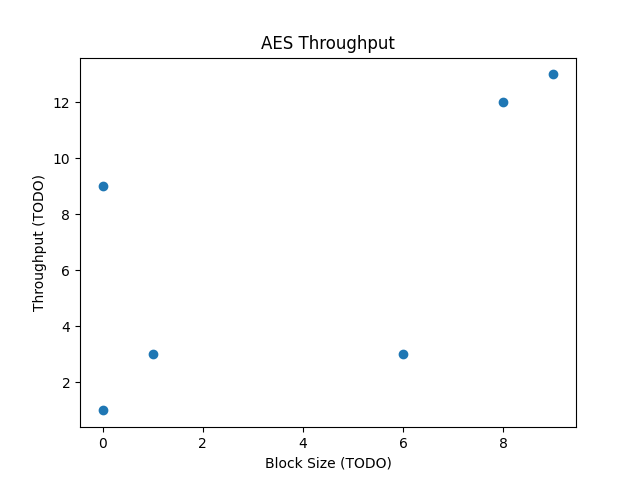
\includegraphics[width=0.8\textwidth]{./plts/aes.png}
	%\caption{}
	\label{fig.1: Performance of AES}
\end{figure}

\begin{figure}
	\centering
	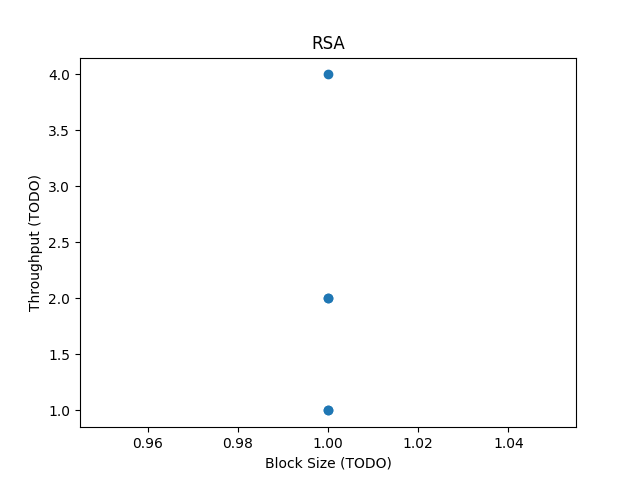
\includegraphics[width=0.8\textwidth]{./plts/rsa.png}
	%\caption{}
	\label{fig.2: Performance of RSA}
\end{figure}

\section*{Questions}
\subsection*{question 1}
\subsection*{question 2}
\subsection*{question 3}

\end{document}
